\documentclass[tikz,multi,border=10pt]{standalone}
\usepackage{color}
\usetikzlibrary{shadows,arrows.meta,positioning,backgrounds,fit}

% Define block styles
\tikzset{%
    materia/.style={draw, fill=blue!20, text width=6.0em, text centered, minimum height=1.5em,drop shadow},
    etape/.style={materia, text width=8em, minimum width=10em, minimum height=3em, rounded corners, drop shadow},
    texto/.style={above, text width=6em, text centered},
    linepart/.style={draw, thick, color=black!50, -LaTeX, dashed},
    line/.style={draw, thick, color=black!50, -LaTeX},
    ur/.style={draw, text centered, minimum height=0.01em},
    back group/.style={fill=yellow!20,rounded corners, draw=black!50, dashed, inner xsep=15pt, inner ysep=10pt},
}

\newcommand{\etape}[2]{node (p#1) [etape] {#2}}

\newcommand{\transreceptor}[3]{%
    \path [linepart] (#2) -- (#1.east);}

\begin{document}
\noindent
\begin{tikzpicture}
\node [anchor=west] (RCNN) at (-2.5, 21) {\Large Faster RCNN};
\node [anchor=west] (SSD) at (-2.5, 15) {\Large SSD};
\node [anchor=west] (YOLOv2) at (-2.5, 9) {\Large YOLOv2};
\node [anchor=west] (RRPN) at (-2.5, 3) {\Large RRPN};



\begin{scope}[xshift=1.5cm]
    \node[anchor=south west,inner sep=0] (image) at (0,0) {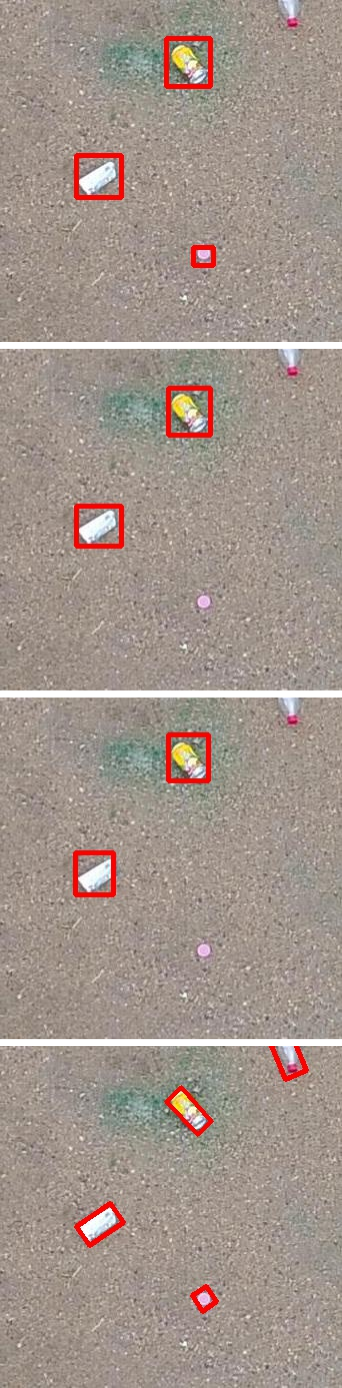
\includegraphics[width=0.5\textwidth]{results/result1.png}};

    \begin{scope}[x={(image.south east)},y={(image.north west)}]
        \draw [-stealth, line width=5pt, cyan] (RCNN) -- ++(0.4,0.0);
        \draw [-stealth, line width=5pt, cyan] (SSD) -- ++(0.565,0.0);
        \draw [-stealth, line width=5pt, cyan] (YOLOv2) -- ++(0.48,0.0);
        \draw [-stealth, line width=5pt, cyan] (RRPN) -- ++(0.52,0.0);
    \end{scope}
\end{scope}

\draw[line width=3pt, blue] (6, 25.5) rectangle (7.5, 23.5);
\draw[line width=3pt, blue] (6, 19.3) rectangle (7.5, 17.3);
\draw[line width=3pt, blue] (6, 13.2) rectangle (7.5, 11.2);
\draw[line width=3pt, blue] (6, 7) rectangle (7.5, 5);

\draw[line width=3pt, blue] (4.5, 19) rectangle (6, 21);
\draw[line width=3pt, blue] (4.5, 13) rectangle (6, 15);
\draw[line width=3pt, blue] (4.5, 6.8) rectangle (6, 8.8);
\draw[line width=3pt, blue] (4.5, 1) rectangle (6, 3);

\end{tikzpicture}%
\end{document}


